\chapter{Introducción y Estado del Arte}
\label{c-intro spanish}

\section{Neurociencia, neuronas y su dinámica}
% \textit{¿Qué son las neuronas, su dinámica y cuáles son las tareas pendientes?}
La neurociencia es un campo amplio y desafiante. Afronta preguntas cruciales, tales como el estudio de los mecanismos neuronales subyacentes a la actividad cerebral, cómo pueden esos mecanismos resultar en la cognición o el comportamiento humano, cómo se procesa y transfiere la información a través de la actividad neuronal, cómo se generan las enfermedades neuronales y cómo podemos detectarlas y tratarlas. 
Estas preguntas y muchas más han sido problemas abiertos que han intrigado a la comunidad científica desde los primeros pasos en el campo. La neurociencia nació como una disciplina a partir de la anatomía, la fisiología, la bioquímica y la biofísica. Debido a la amplitud del campo, se suele abordar desde distintas perspectivas y comunmente se le hace referencia por sus subcampos, por ejemplo, Neurobiología, Neurofarmacología, Neurociencia Clínica, Neurociencia del Desarrollo, Neurociencia de Sistemas, Neurociencia Cognitiva, Neurociencia Computacional, Neurotecnología, etc. Todos estos campos tienen como objetivo explicar o reparar la función cerebral, ya sea en su totalidad o en partes. Utilizan diferentes técnicas y enfoques, algunos de los cuales dan lugar a campos completamente nuevos, como la Neuroimagen.

No podemos pensar o discutir sobre neurociencia sin destacar el trabajo de Santiago Ramón y Cajal, crucial en los primeros pasos para comprender el cerebro \parencite{ramonycajal_textura_1899,decarlos_historical_2007,decastro_editorial_2016,delgado-garcia_cajal_2015,decastro_cajal_2019}. La idea de la "doctrina de la neurona" fue un impulso en el estudio del cerebro, explicando y describiendo la estructura de células individuales llamadas \textit{neuronas} que son capaces de conectarse y, por lo tanto, comunicarse mediante \textit{sinapsis}. La Figura \ref{fig:cajal-neuron spanish} muestra uno de los dibujos de Cajal que ilustra la retina de la abeja y una primera aproximación al posible curso de las corrientes en ella.

\begin{figure}[htb!]
    \centering
    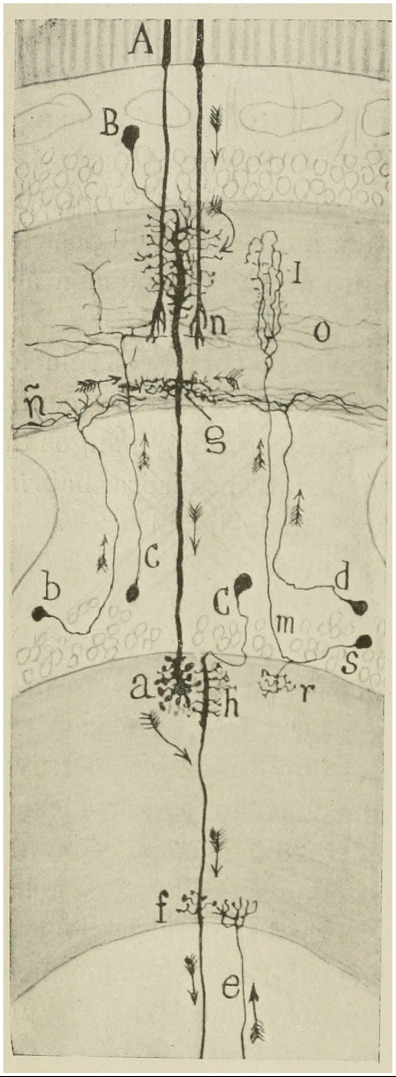
\includegraphics[width=0.3\textwidth]{img/intro/cajal-flow_small.jpg}
    % https://es.wikipedia.org/wiki/Doctrina_de_la_neurona#/media/Archivo:CajalCerebellum.jpg
    % https://microbioblog.es/la-fascinante-historia-de-la-reazione-nera
    \caption{Ilustración de Ramón y Cajal que muestra el probable curso de las corrientes en la retina de la abeja. (A) bastones; (B) segunda neurona visual (monopolar gigante); (C) corpúsculo ganglionar (tercera neurona visual); (B,C) centrífugas cortas; (M,S) célula T o célula de conexión interzonal; (F,G) dendritas basales destinadas a articularse con fibras centrífugas (Ramón y Cajal y Sánchez, 1915). Copyright Serrano-Herrera y Espinosa-Sánchez from \textcite{serrano-herrera_domingo_2024} (\href{https://creativecommons.org/licenses/by-sa/4.0/}{CC BY-SA 4.0})}
    \label{fig:cajal-neuron spanish}
\end{figure}
%Desde ese punto de partida ha habido hallazgos importantes en los tipos y estructuras de neuronas, como las células gliales \ref{}.

El cerebro es un sistema complejo que podemos estudiar desde diferentes prismas. En esta tesis, seguimos un enfoque \textit{bottom-up} (de abajo hacia arriba), en el que analizamos de forma experimental y teórica la actividad neuronal en canales iónicos y en pequeños circuitos (con pocas sinapsis). Además, seguimos una perspectiva neurocomputacional basada en el procesamiento secuencial jerárquico de la información, que se definirá en detalle en la subsección \ref{sec:computational neuroscience spanish}. En las siguientes líneas abordaremos las bases de la activación neuronal desde una perspectiva computacional necesaria para la comprensión de este documento. Nos centraremos no en sus propiedades moleculares sino en el cambio de voltaje que son capaces de producir y cómo eso interopera para dar lugar a la actividad neuronal.


\subsection{Dinámica neuronal}
Las neuronas son células morfológicamente compuestas por dendritas, donde se reciben las conexiones de otras neuronas a través de sinapsis, un soma o cuerpo celular (donde típicamente se integra la información) y un axón (donde la información se transmite como salida). Dado que las neuronas son las células que presentan la mayor diversidad en morfología. Aunque esta descripción no se aplica a todos los tipos neuronales, nos sirve para comenzar a resaltar la importancia de las escalas espaciales en el sistema nervioso.

% Como se mencionó, hay muchas formas diferentes de estudiar la dinámica neuronal, pero un descriptor común de la actividad neuronal son los potenciales de acción. Los potenciales de acción son el
La actividad eléctrica neuronal a menudo se describe en términos de la evolución del voltaje de la membrana causada por el flujo de canales iónicos entre el interior y el exterior de la célula \parencite{kandel_principles_2012}. El cambio rápido característico en el voltaje de la membrana cuando una neurona emite una señal de salida se llama potencial de acción o \textit{spike}. Estas suelen considerarse unidades mínimas de información para la recepción, procesamiento y transmisión llevadas a cabo por las neuronas. Una definición más concreta de \textit{spike} podría ser "un cambio abrupto y transitorio del voltaje de la membrana que se propaga a otras neuronas a través de una larga protusión llamada axón" \parencite{izhikevich_dynamical_2007}. Así, cuando no se reciben entradas, el potencial de la membrana de una neurona es negativo y se llama potencial de reposo. Cuando este potencial se altera por una entrada que hace que el voltaje aumente, se conoce como despolarización. Después de alcanzar un pico de voltaje, típicamente un valor positivo de alrededor de 40mV, el potencial comienza a disminuir nuevamente. Cuando el potencial es más negativo que el potencial de reposo, se conoce como hiperpolarización. La Figura \ref{fig:action potential spanish} ilustra las fases secuenciales de la generación del potencial de acción.

\begin{figure}[htb!]
	\centering
	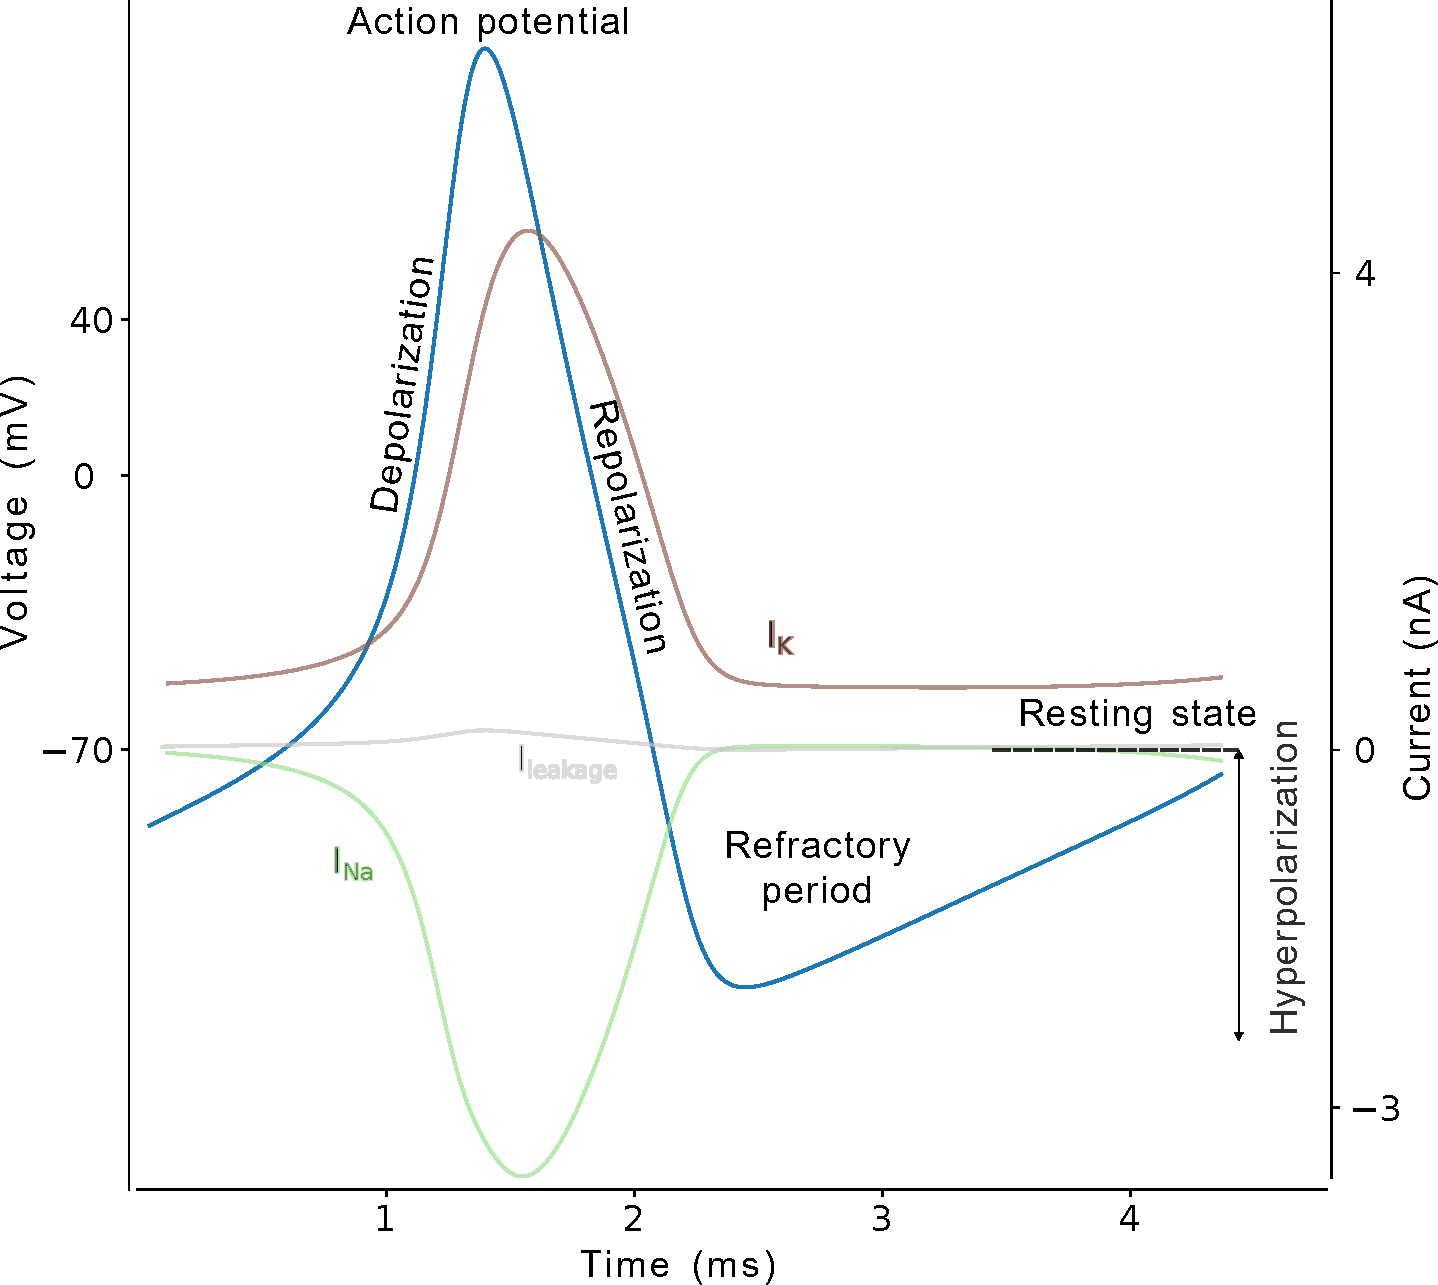
\includegraphics[width=0.8\textwidth]{img/intro/action_potential.pdf}
	\caption{Representación de las fases secuenciales y terminología de un potencial de acción. (Adaptado de Chris73, Wikimedia Commons, \href{https://creativecommons.org/licenses/by-sa/3.0/}{CC BY-SA 3.0}). En cada una de estas fases de la generación del potencial de acción, se activan secuencialmente diferentes canales iónicos, por ejemplo, el canal de sodio está involucrado durante la fase de despolarización y su actividad disminuye a medida que el canal de potasio se activa principalmente en la fase de repolarización.}
	\label{fig:action potential spanish}
\end{figure}

La actividad neuronal se genera por el flujo de diferentes canales iónicos que contrarrestan el valor del voltaje generando el potencial de acción \parencite{koch_biophysics_1999}. La membrana puede estar compuesta por diferentes canales iónicos, y su dinámica está condicionada por esa combinación y las posibles conexiones sinápticas. Estos cambios en la dinámica pueden manifestarse de diferentes maneras, pero las más notorias son la forma y la evolución temporal del potencial de acción. %p61 The Neuron
Por ejemplo, en la Fig. \ref{fig:spike-types spanish} hay un ejemplo de dos potenciales de acción distintos con diferencias visibles en su forma, uno de ellos presenta una forma simétrica, donde las pendientes de despolarización y repolarización son similares, mientras que en la forma de onda de la derecha, hay un notable hombro en la repolarización y su escala temporal es casi el doble en comparación con el ejemplo mostrado en (a).

\begin{figure}[htb!]
	\centering
	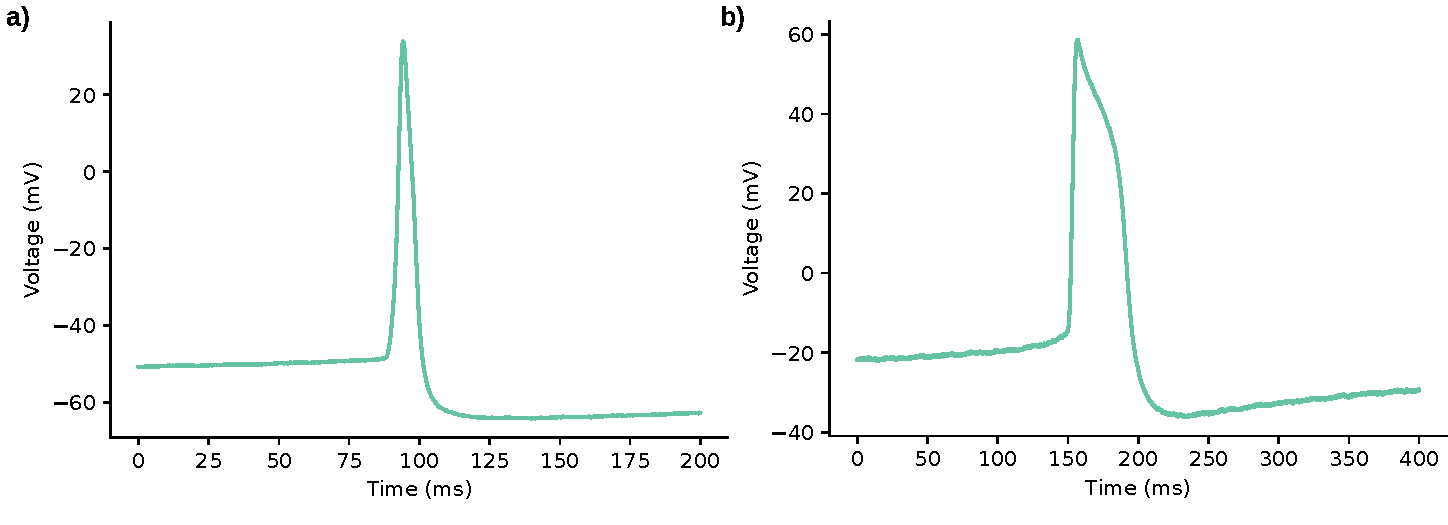
\includegraphics[width=\linewidth]{img/intro/spike-types.pdf}
	\caption{Ejemplos de diferentes formas de picos. Representación de dos grabaciones de dos células diferentes en el ganglio parietal derecho de \textit{Lymnaea stagnalis}. Izquierda: pico simétrico; derecha: pico con forma de hombro.}
	\label{fig:spike-types spanish}
\end{figure}

Si los picos se consideran las piezas mínimas de información al codificar la actividad neuronal, la combinación de estas piezas mínimas de información lleva a nuevas formas de información, también conocidas como ráfagas. Aunque no hay una descripción fija de una ráfaga, y dependiendo del animal y el sistema una ráfaga puede verse diferente \parencite{russell_bursting_1978,palmu_detection_2010,lundqvist_gamma_2016}, hay algunas características comunes en las ráfagas: típicamente consisten en un grupo de \textit{spikes} (más de dos) sobre una despolarización sostenida, y estos grupos están separados por un período de quiescencia de hiperpolarización llamado intervalo entre ráfagas (IBI). La Figura \ref{fig:spike_activity-types spanish} muestra varios ejemplos de distintas actividades neuronales observadas en grabaciones intracelulares. Dependiendo de la neurona específica y el circuito, las neuronas pueden presentar disparo tónico (primera columna), a diferentes velocidades, o actividad en ráfagas (segunda columna).

\begin{figure}[htb!]
	\centering
	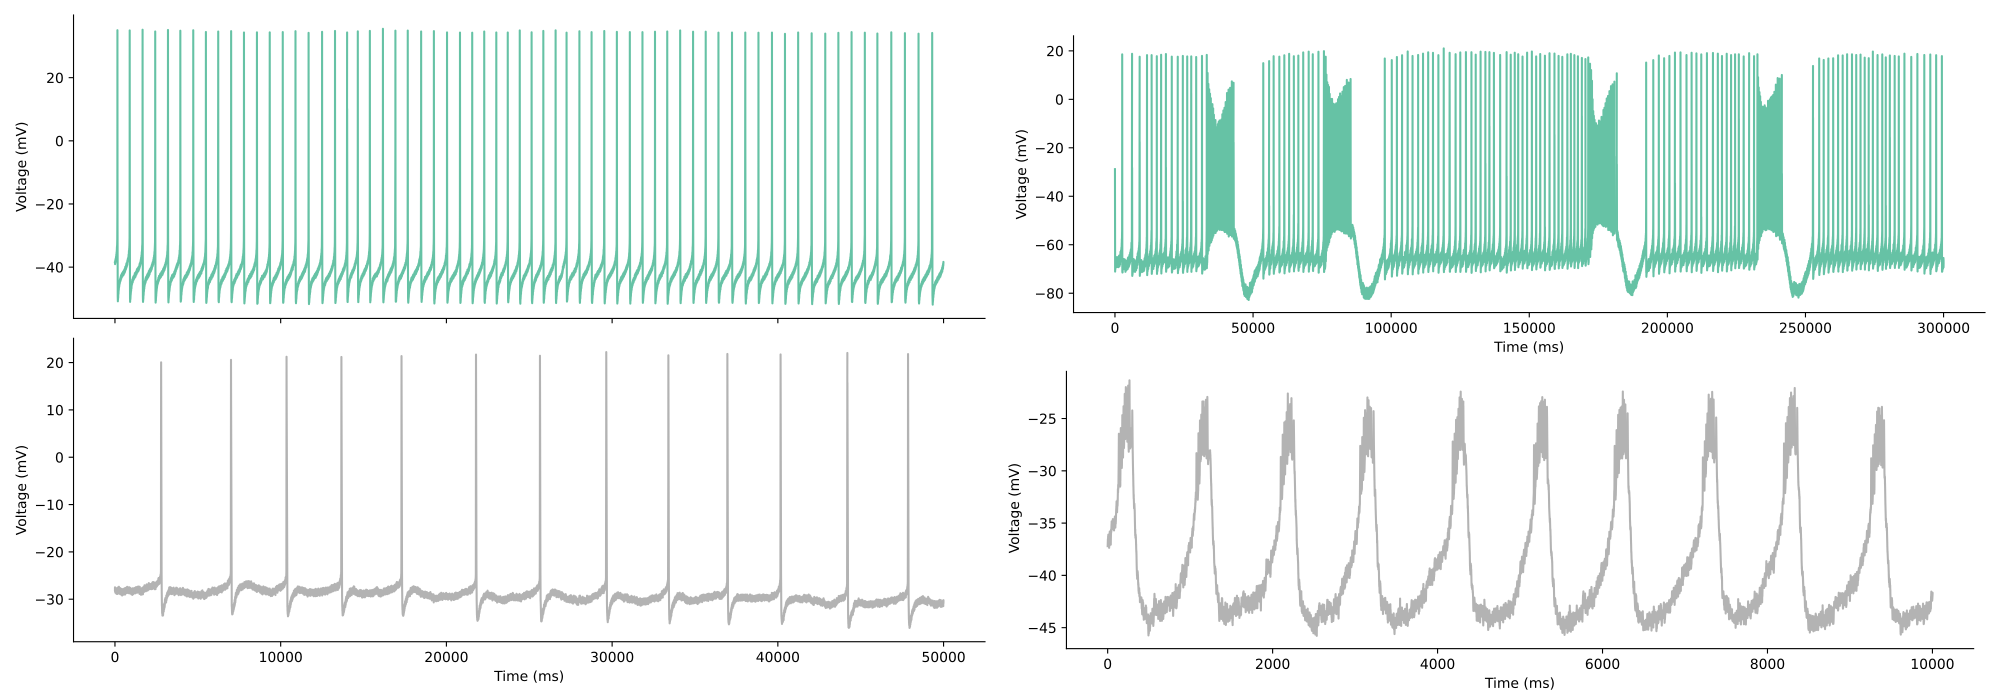
\includegraphics[width=\linewidth]{img/intro/spike_activity-types.png}
	\caption{Representación de dos ejemplos de diferentes actividades neuronales de disparo. Izquierda: dos grabaciones intracelulares simultáneas en \textit{Lymnaea stagnalis} mostrando disparo tónico a dos frecuencias diferentes. Derecha: Dos ejemplos de actividad en ráfagas, de registros intracelulares en \textit{Lymnaea stagnalis} (panel superior) y en \textit{Carcinus maenas} (panel inferior).}
	\label{fig:spike_activity-types spanish}
\end{figure}

Tradicionalmente, los códigos neuronales se han estudiado centrándose en la activación de \textit{spikes} individuales, por ejemplo, mediante la binarización de la actividad (la neurona genera un pico o no). Las ráfagas también pueden ser informativas en términos de la actividad neuronal, ya sea como una pieza completa de información o como una caja de datos compleja en sí misma: "las ráfagas son una familia de patrones de disparo que desencadenan mecanismos fisiológicos que no se activan con el mismo número de \textit{spikes} en relativo aislamiento" \parencite{friedenberger_silences_2023}. Las ráfagas pueden originarse por activación interna, principalmente por canales de calcio o por la dinámica sináptica que involucra a la célula correspondiente (inhibición/excitación) (para una revisión extendida ver \parencite{friedenberger_silences_2023}). Este es el caso en muchos Generadores Centrales de Patrones (CPGs) \parencite{katz_evolution_2016,steuer_central_2018}, que se discutirán en detalle a continuación y en el Capítulo \ref{c-invariants}.

\subsection{Dinámicas de redes}

Aunque el análisis de la actividad de una sola neurona es importante para caracterizar su dinámica, cuando se habla de procesamiento de información y comportamiento, también es crucial estudiar la dinámica general del circuito. Un circuito de neuronas se define por células nerviosas interconectadas por sinapsis. Existen dos tipos principales de sinapsis en el sistema nervioso: conexiones eléctricas y químicas, como se muestra en la Fig. \ref{fig:synapse-types spanish}. La principal diferencia entre ellas radica en cómo se lleva a cabo la comunicación. Las sinapsis químicas ocurren mediante la mediación de \textit{neurotransmisores}, donde una neurona presináptica libera estas moléculas que se unen a los neuroreceptores para producir una alteración en la neurona postsináptica. Por lo tanto, esta conexión es asimétrica y unidireccional, mientras que en las sinapsis eléctricas encontramos una conexión simétrica y bidireccional. En estas sinapsis, las neuronas están casi unidas por una estructura llamada \textit{unión gap} (\textit{gap junction} en inglés), que conecta ambas neuronas en una estructura tisular que limita la fuga al espacio extracelular. Esta comunicación permite que la carga eléctrica fluya de una neurona a otra y es más rápida que las sinapsis químicas, que, en comparación, no tienen retraso. La actividad de las neuronas acopladas eléctricamente suele ser sincrónica \parencite{levitan_neuron_2002}.

\begin{figure}[hbt!]
	\centering
	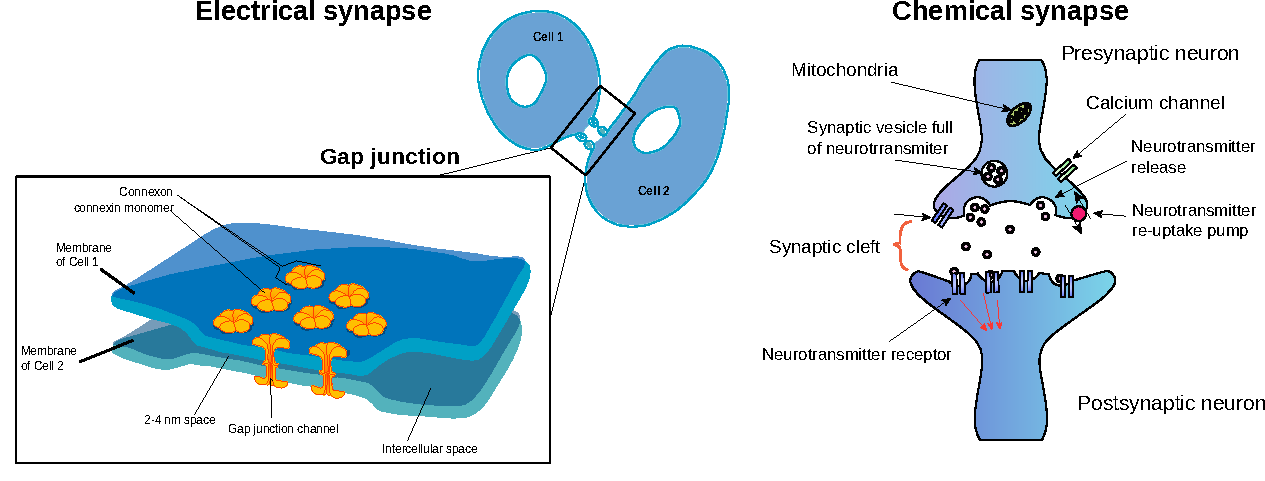
\includegraphics[width=\linewidth]{img/intro/synapses.pdf}
	\caption{Representación de tipos de sinapsis. Izquierda: Ejemplo de sinapsis eléctrica entre dos células y diagrama de unión estrecha (Adaptado de \href{https://commons.wikimedia.org/wiki/File:Gap_cell_junction-en.svg}{Wikimedia Commons}). Derecha: Ejemplo de estructura de sinapsis química (Adaptado de \href{https://commons.wikimedia.org/wiki/File:Synapse_diag1.svg}{Wikimedia Commons})}
	\label{fig:synapse-types spanish}
\end{figure}

En los circuitos neuronales, las células pueden estar conectadas por uno o ambos tipos de sinapsis químicas y eléctricas, y generalmente también están conectadas a otros circuitos o neuronas moduladoras. La Figura \ref{fig:neural circuits spanish} ilustra dos ejemplos de circuitos a nivel celular y macroscópico. En este contexto, se forman sistemas complejos de redes de redes, que pueden funcionar a diferentes escalas temporales y pueden participar en una o varias funcionalidades. Esta interconexión de redes y, a un nivel más bajo, de células, conduce a activaciones secuenciales y transferencias de acciones en secuencias de secuencias.

\begin{figure}[hbt!]
	\centering
	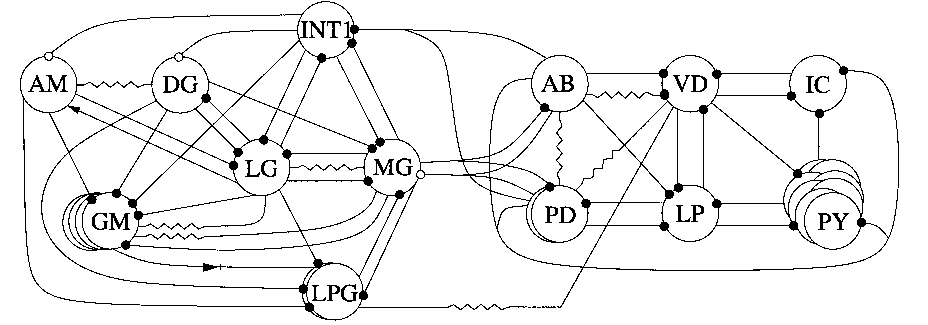
\includegraphics[width=0.64\textwidth]{img/intro/cpg diagram.png}
	\includegraphics[width=0.35\textwidth]{img/intro/The_Human_Connectome.png}
	\caption{Izquierda: Esquema del circuito gástrico y pilórico de \textit{Carcinus Maenas} \parencite{huerta_topology_2001}. Derecha: Conectoma en el cerebro humano renderizado a partir de 20 sujetos (Por Andreashorn - Trabajo propio,\href{https://commons.wikimedia.org/w/index.php?curid=41581320}{CC BY-SA 4.0})}
	\label{fig:neural circuits spanish}
\end{figure}

\section{La naturaleza secuencial de la dinámica neuronal}

Las dinámicas cerebrales pueden describirse como secuencias de interacciones, desde moléculas, hasta neuronas, movimientos motores y comportamiento, dentro de una jerarquía coordinada de escalas temporales y espaciales \parencite{kiebel_hierarchy_2008,yuste_cortex_2005,rabinovich_discrete_2018,rabinovich_neurons_2023}, desde activaciones de canales iónicos hasta codificación sensorial, procesamiento y toma de decisiones. Su estudio revela aspectos fundamentales de la función cerebral y la cognición, por ejemplo, la transmisión de impulsos, la función ejecutiva, el procesamiento espacial o la memoria.

Un ejemplo común de procesamiento secuencial es el habla, donde los patrones secuenciales están presentes en la estructura de las frases, como secuencias de secuencias de sílabas, palabras y silencios \parencite{kiebel_recognizing_2009}. En esta línea, un caso de estudio extendido es el canto de los pájaros, que tiene similitud con el habla humana, ya que involucran secuencias de sonidos coordinados \parencite{prather_brains_2017,fishbein_sound_2019}. Aparte de en el habla, el procesamiento secuencial también está presente en el movimiento motor, desde la activación muscular hasta acciones coordinadas repetitivas como el golpeteo rítmico o la interpretación musical \parencite{ding_temporal_2017}. Además, hay muchos procesos cognitivos importantes que dependen de mecanismos secuenciales como la percepción, la memoria, la toma de decisiones, la atención y la emoción \parencite{varona_hierarchical_2016, he_robust_2018, rabinovich_sequential_2020}.

Sin embargo, no está claro cómo procesa exactamente el cerebro el tiempo. En contraste con la teoría de un reloj central que gestiona el tiempo para cada tarea conductual, la teoría de un procesamiento temporal distribuido \parencite{buonomano_temporal_1995,ivry_representation_1996} es bien aceptada. En este marco, especialmente en la coordinación del movimiento, existe la necesidad de circuitos que gestionen la actividad rítmica secuencial. Este es el caso de los Generadores Centrales de Patrones (CPGs), circuitos de neuronas con topología cerrada que activan secuencialmente neuronas y generan actividad motora coordinada \parencite{selverston_reliable_2000}. Están presentes en muchos sistemas, desde insectos hasta humanos \parencite{pearson_central_1972,marder_central_2001,mackay-lyons_central_2002,minassian_human_2017}. Hay varios aspectos clave que hacen de estos circuitos un caso de estudio interesante. Primero, sus neuronas están organizadas en topologías cerradas recibiendo retroalimentación de células compañeras \parencite{huerta_topology_2001}. Estos circuitos pueden mantener una actividad rítmica de manera autónoma, típicamente mediante interacciones inhibitorias mutuas \parencite{katz_evolution_2016}. Segundo, su actividad es lo suficientemente flexible como para adaptarse a cambios en el contexto, por ejemplo, variaciones en el terreno al caminar. Finalmente, están presentes en muchos sistemas y en algunos de ellos hay una relación directa entre la actividad de las neuronas en el circuito y el movimiento motor que producen. Por ejemplo, en el CPG estomatogástrico en el cangrejo \textit{C. maenas}, encargado del movimiento del píloro, las neuronas PD (dilatador pilórico), LP (pilórico lateral) y PY (PYlórico) corresponden a la dilatación del píloro, el cierre del píloro y la contracción del constrictor rostral para mover los alimentos en el sistema digestivo \parencite{moulins_introduction_1987,selverston_oscillations_2006}.

\begin{figure}[hbt!]
	\centering
	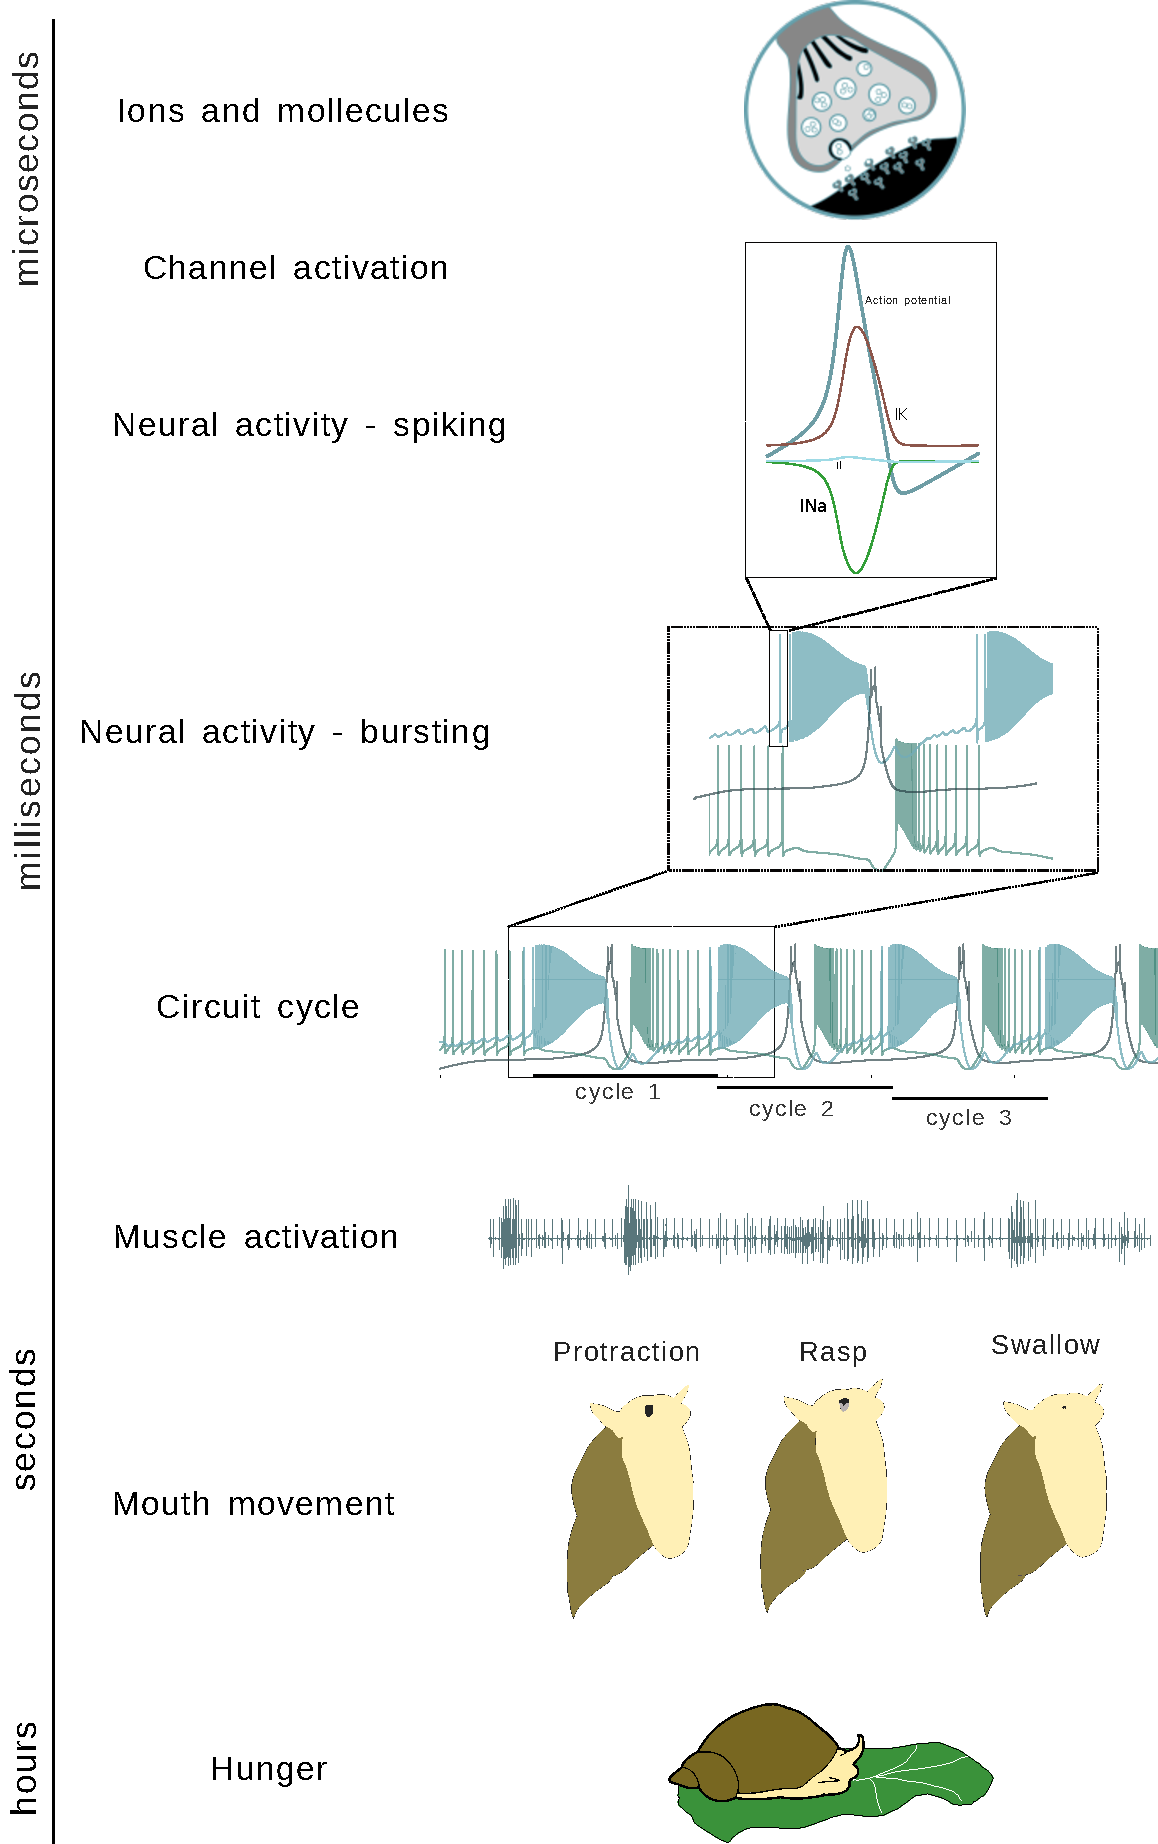
\includegraphics[width=0.7\textwidth]{img/intro/time scale/time-scale-feeding.pdf}
	\caption{Ilustración del proceso de alimentación secuencial en diferentes escalas de tiempo en {\sl Lymnaea stagnalis}.}
	\label{fig:time-scale feeding spanish}
\end{figure}

La actividad secuencial en el cerebro va desde la escala de sub-milisegundos hasta días (la escala temporal de los ritmos circadianos \parencite{mauk_neural_2004}). La Figura \ref{fig:time-scale feeding spanish} muestra un ejemplo ilustrativo de la naturaleza secuencial de la actividad neuronal en diferentes escalas en la generación de actividad motora coordinada en la alimentación de un caracol. A la escala de sub-milisegundos, hay un flujo de iones que genera una secuencia de activación de canales iónicos, que en la escala de milisegundos produce potenciales de acción. La combinación de ellos en forma de ráfagas rítmicas, activa los músculos correspondientes en la escala de segundos y genera el movimiento secuencial necesario para alimentarse: abrir la boca, raspar el alimento y tragar, que se repite a lo largo del día.

El estudio de la dinámica de los potenciales de acción y la interacción entre los canales iónicos y las sinapsis es crucial, ya que es una parte clave en cualquier proceso cerebral, y no puede separarse del estudio de la actividad en su conjunto. La alteración de la dinámica de estos canales a diferentes niveles, puede afectar las entradas/salidas sinápticas, cómo se comunican las neuronas y el proceso resultante. Los canales iónicos son el punto de partida de las señales eléctricas subyacentes a la actividad de la red neuronal, y su mal funcionamiento puede contribuir a trastornos neuronales \parencite{kecskes_editorial_2023}. Por lo tanto, comprender la actividad cerebral no solo a gran escala sino también desde la etapa de generación de dinámicas de voltaje puede ser clave para una comprensión realmente completa de los sistemas neuronales. Su estudio también puede ayudar a distinguir entre la modulación a corto y largo plazo, un aspecto clave en la plasticidad neuronal y la aplicación de técnicas neuromoduladoras \parencite{chambers_lightactivated_2008,burke_modulation_2019}.

Es importante explorar los mecanismos que permiten mantener una actividad secuencial robusta a pesar de los cambios en el contexto y la variabilidad subyacente en la dinámica neuronal. Los potenciales de acción y las ráfagas pueden clasificarse según su forma de onda y la actividad de disparo agrupada. Sin embargo, en esos subgrupos hay una alta intra-variabilidad, donde, por ejemplo, la actividad de ráfagas puede diferir en forma y duración, es decir, en el número de picos en una ráfaga. La Figura \ref{fig:burst variability spanish} muestra un ejemplo de la variabilidad en la forma de onda y la duración de la ráfaga para una secuencia de varias ráfagas.

\begin{figure}[htb!]
	\centering
	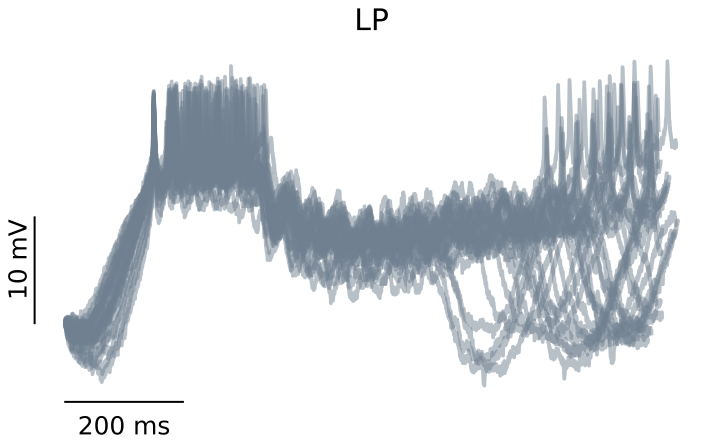
\includegraphics[width=0.6\textwidth]{img/intro/burst_variability.png}
	\caption{Superposición de ráfagas en diferentes instantes de tiempo alineadas por el primer \textit{spike} en la ráfaga para grabaciones intracelulares de una neurona LP en el CPG estomatogástrico.}
	\label{fig:burst variability spanish}
\end{figure}

El estudio de esta variabilidad revela factores clave en la secuencialidad y cómo se mantiene a pesar de diferentes modulaciones intrínsecas o externas. Este es el caso, por ejemplo, de los invariantes dinámicos secuenciales, es decir, relaciones robustas entre intervalos de tiempo que conforman una secuencia neuronal, al analizar la actividad ciclo a ciclo \parencite{reyes_artificial_2008,elices_robust_2019,garrido-pena_characterization_2021,berbel_emergence_2024}. Estos invariantes dinámicos secuenciales pueden tener un papel crucial para entender la coordinación de la actividad secuencial y el equilibrio entre la robustez y la flexibilidad requerida para una función efectiva en muchos procesos cerebrales \parencite{tatsuno_analysis_2015,ullen_neural_2003,zimnik_independent_2021,zhou_neural_2020,dragoi_cell_2020}. Discutiremos en detalle este fenómeno en el CPG alimentario de \textit{Lymnaea stagnalis} en el capítulo \ref{c-invariants}.\\


\section{Estudiando la dinámica neuronal en modelos computacionales.}
\label{sec:neurociencia_computacional}
La Neurociencia Computacional es un subcampo de la neurociencia que utiliza técnicas teóricas y computacionales para abordar el estudio del sistema nervioso en múltiples niveles, desde el nivel molecular hasta las complejas redes que dan forma al comportamiento. Es, por lo tanto, un campo multidisciplinario. La base de la Neurociencia Computacional radica en la comprensión de la dinámica cerebral a partir de sus señales eléctricas y la información que transportan \parencite{schwiening_brief_2012,catterall_hodgkinhuxley_2012,dimitrov_information_2011,shannon_mathematical_1948}. La Neurociencia Computacional ha ampliado su alcance, llevando a nuevos caminos de investigación que incluyen redes complejas, teoría de grafos, análisis de células individuales y técnicas de aprendizaje automático \parencite{cns2023}. En campos como la Inteligencia Artificial incluso existe una relación simbiótica entre ambos, en la que se inspiran y se ayudan mutuamente a crecer \parencite{amunts_human_2019,wozniak_deep_2020,goncalves_training_2020}.

Una parte importante de la Neurociencia Computacional es la descripción de sistemas neuronales con modelos teóricos y la reproducción de fenómenos clave mediante la simulación del modelo. La simulación de la actividad neuronal es una herramienta de gran potencial para explorar la dinámica neuronal, sus fuentes biofísicas, los posibles mecanismos subyacentes en la señal neuronal y el complejo procesamiento de la información observada. Su fuerza radica en la completa accesibilidad a las variables del modelo, el rango típicamente extenso de parámetros ajustables en el modelo que se pueden explorar y la capacidad para evaluar el papel de elementos distintos en el sistema o circuito incluyéndolos o excluyéndolos de las simulaciones. Aunque los modelos no pueden sustituir completamente la investigación en sistemas vivos, sí nos acercan a la comprensión de la dinámica neuronal compleja, siendo una alternativa rápida, eficaz y de bajo costo para los avances científicos. Además, los modelos son un complemento esencial para la neurociencia experimental, alcanzando descripciones detalladas donde los enfoques experimentales como la electrofisiología tienen limitaciones debido a la observabilidad parcial subyacente.

Los modelos pueden clasificarse según su nivel de descripción, es decir, qué nivel de simplificación/abstracción se utiliza, el detalle de la estructura/fenómeno que se modela y el tamaño de la red, o su capacidad para reproducir la actividad neuronal observada, por ejemplo, dinámicas caóticas. La Figura \ref{fig:models-classification spanish} ilustra este tipo de clasificación, con ejemplos de modelos de grandes redes como \textcite{potjans_celltype_2014,bezaire_interneuronal_2016}, de células individuales pero aún detallados como en \textcite{smith_dendritic_2013}, y descripciones más abstractas como la propuesta en \textcite{izhikevich_simple_2003}. En cuanto al nivel de descripción, en los diferentes modelos biofísicos siempre hay una elección entre la descripción detallada de las no linealidades, canales y propiedades de excitación, y la eficiencia en la computación. En esta línea, los investigadores pueden elegir entre modelos basados en conductancia \parencite{hodgkin_quantitative_1952}, ricos en la descripción de no linealidades, o modelos dinámicos simplificados \parencite{hindmarsh_model_1984,fitzhugh_impulses_1961}, que típicamente representan no linealidades con simplificaciones polinomiales (ver \parencite{torres_modeling_2012} para una revisión de diferentes niveles de modelado neuronal).

\begin{figure}[bth!]
\centering
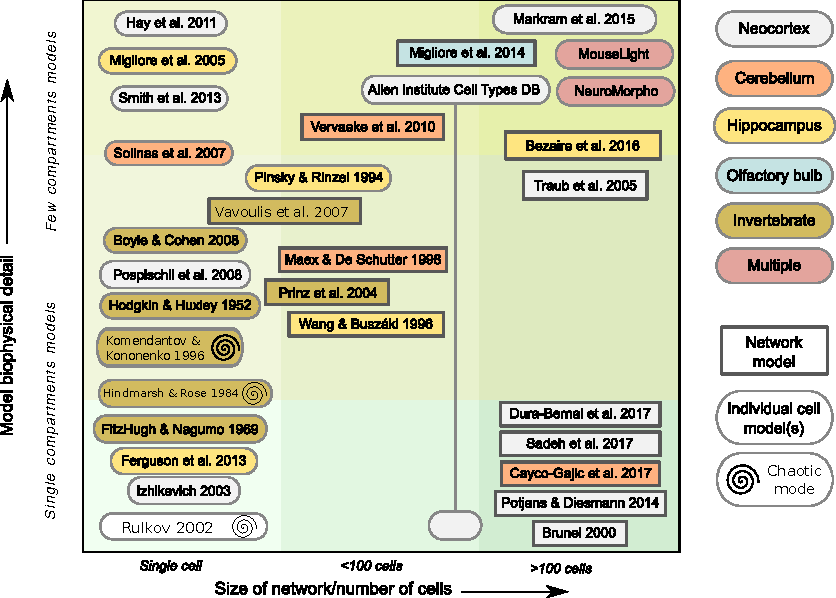
\includegraphics[width=\textwidth]{img/intro/models classification_v2.pdf}
\caption{Modelos neuronales y de red clasificados por detalle biofísico, estructura modelada y tamaño de la red. Figura adaptada de la Fig. 2 \parencite{gleeson_open_2019} bajo licencia \href{http://creativecommons.org/licenses/by/4.0/}{Creative Commons CC-BY}. Los modelos están clasificados por el detalle biofísico, siendo los modelos en la parte inferior los menos específicos; por el tamaño de la red modelada, de izquierda a derecha, una célula a cientos de células; y por la estructura cerebral que modelan, representada en cajas de colores. La forma de la caja también clasifica en modelo de red o célula individual. Se incluyó una tercera categoría a partir del trabajo original, representada por una espiral en la caja, que indica la capacidad del modelo para producir actividad caótica sin alteraciones externas, es decir, reproducir variabilidad intrínseca espontánea. Aunque la figura no contiene todos los enfoques de modelos, ilustra hitos clave en el modelado neuronal.}
\label{fig:models-classification spanish}
\end{figure}

\subsection{Modelos basados en conductancia}

En esta tesis, todos los registros experimentales se han apoyado en simulaciones con modelos basados en conductancia. Se definen como descripciones matemáticas de la dinámica de los canales iónicos, basadas en su conductancia dependiente del voltaje. El estudio pionero de \textcite{hodgkin_quantitative_1952} definió ecuaciones dinámicas basadas en el circuito eléctrico equivalente de las propiedades eléctricas de las neuronas en el axón gigante del calamar, ver Fig. \ref{fig:electrical circuit spanish}. Este circuito modelado también se utiliza para conformar la configuración de registro intracelular, donde la pipeta se incluye como una corriente adicional compensada por el electrodo en la solución (ver Fig. \ref{fig:clamp circuit spanish}).

\begin{figure}[htb!]
\centering
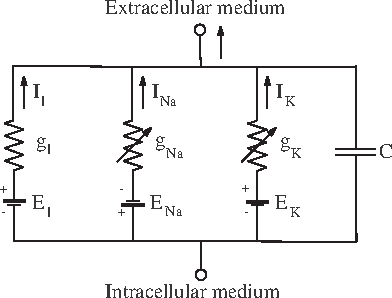
\includegraphics[width=0.7\textwidth]{./img/intro/electrical_circuit.pdf}
\caption{Circuito eléctrico que describe el potencial de membrana en un modelo de neurona basado en conductancia.}
\label{fig:electrical circuit spanish}
\end{figure}

\begin{figure}[htb!]
\centering
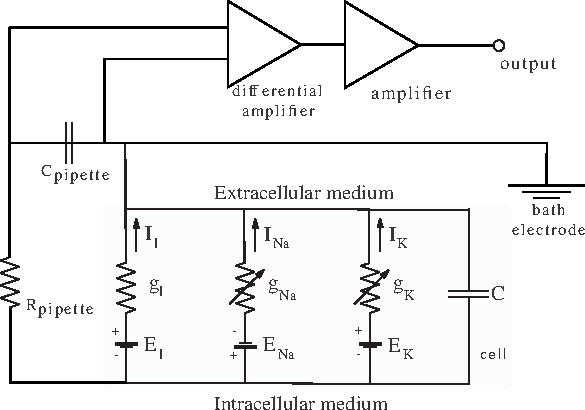
\includegraphics[width=0.7\textwidth]{./img/intro/intracellular_recording_circuit.pdf}
\caption{Circuito eléctrico que representa el esquema para registros intracelulares.}
\label{fig:clamp circuit spanish}
\end{figure}

En estos modelos, la simulación de la actividad eléctrica neuronal se basa en la descripción matemática de diferentes canales iónicos en el circuito, cuya dinámica también está bien definida por compuertas de activación. Primero, hay una descripción matemática de la dependencia del voltaje en el tiempo, como se describe en la ecuación \ref{eq:voltage ions spanish}:

\begin{equation}
C_m \frac{dV}{dt} = I - \sum I_{x},
\label{eq:voltage ions spanish}:
\end{equation}

donde \( V \) es el potencial de membrana, \( I \) es una corriente externa, por ejemplo, un estímulo externo o una corriente sináptica, \( I_{x} \) es la descripción de la corriente para cada canal involucrado en la generación del potencial de acción, por ejemplo, sodio, potasio, calcio (\( I_K \), \( I_{Na} \), \( I_{Ca} \)).

En segundo lugar, cada canal también se describe dependiente del voltaje compuesto por dinámicas de compuertas de activación:

\begin{equation}
I_x =  g_x m^n h^n (V - E_x),
\end{equation}

donde \( g_x \) es la conductancia correspondiente del canal, \( E_x \) es el potencial de reversión para ese canal y \( m \) y \( h \) representan las variables de activación e inactivación, respectivamente.
Las compuertas de activación suelen tener una tendencia exponencial y están definidas por dinámicas de activación e inactivación, también dependientes del voltaje y el tiempo. Siguen la estructura en la ecuación \ref{eq:alpha-beta spanish}:

\begin{equation}
\frac{dm}{dt} = \frac{m_{\infty} - m}{\tau_m}
\label{eq:alpha-beta spanish}
\end{equation}

\section{Estudios de animales vertebrados e invertebrados}
\label{c-intro-invertebrates spanish}
El estudio de la dinámica neuronal y el comportamiento se lleva a cabo utilizando muchos modelos animales diferentes. Aparte de los modelos dominantes de roedores, ha habido hallazgos de valor incalculable utilizando invertebrados, como en genética y biología del desarrollo en \textit{C. elegans} \parencite{brenner_genetics_1974}, \textit{pececillos} \parencite{streisinger_production_1981} y \textit{Drosophila} \parencite{nusslein-volhard_mutations_1980}; dinámica neuronal en \textit{Aplysia} \parencite{wachtel_direct_1967} o \textit{Loligo} \parencite{hodgkin_quantitative_1952}, actividad motora en \textit{Panulirus} \parencite{selverston_stomatogastric_1976} y \textit{Carcinus maenas} \parencite{eisen_mechanisms_1982} o \textit{Lymnaea stagnalis} \parencite{benjamin_centraldecastro}, el principal modelo animal en esta tesis. Además de estos ejemplos, estos modelos animales se han utilizado en una amplia variedad de campos, incluidos estudios conductuales, ecotoxicología, evolución, modelado de enfermedades humanas, etc. \parencite{romanova_animal_2018}.

A pesar de las diferencias cerebrales entre invertebrados y mamíferos, existen muchas características universales de los sistemas nerviosos que pueden extrapolarse a los humanos. Debemos tener en cuenta que cualquier modelo animal sigue siendo un marco de investigación, con diferencias respecto al enfoque real de estudio --el cerebro humano-- y como modelo, existen diferencias en la estructura, incluso dentro de las especies de mamíferos \parencite{preuss_taking_2000}. Por lo tanto, mediante el uso de modelos computacionales o explorando más especies animales, se puede establecer una verdad fundamental para los aspectos que conforman la dinámica neuronal y del comportamiento.

Los hallazgos en invertebrados no alcanzan la misma relevancia en muchas ocasiones, a menudo bajo la excusa de que las características en los invertebrados no pueden extrapolarse a los humanos. Sin embargo, los modelos de invertebrados han demostrado su utilidad no solo en la ciencia básica. Podemos encontrar ejemplos de esto en enfermedades humanas, memoria, actividad motora y neuromodulación. Particularmente, en el estudio de procesos neuronales, la facilidad de accesibilidad y el número finito de grandes neuronas en el sistema han hecho de los invertebrados un caso de estudio interesante.

Entre las ventajas de usar invertebrados, vale la pena mencionar el fácil acceso al sistema nervioso y la duración de la actividad espontánea después de la disección durante horas, la facilidad de cría y reproducción o la simplicidad de sus características biológicas, que hacen posible una descripción completa de ellas, como la descripción genómica de \textit{C. elegans} o el sistema nervioso en \textit{Lymnaea stagnalis}. Además, algunas especies seleccionadas fueron un campo principal de estudio en las últimas décadas, por lo que hay una gran cantidad de literatura para cada una, incluso en diferentes campos. Además, a pesar de la simplicidad de estos sistemas, su sistema nervioso sigue siendo capaz de generar actividad neuronal secuencial robusta, comportamiento automático e incluso procesos de aprendizaje.

Aparte de los posibles avances en la ciencia desde un punto de vista productivista, los modelos de invertebrados también pueden cerrar la brecha entre recursos y ciencia, permitiendo que los laboratorios y países de bajos ingresos \textit{hagan} ciencia. Estos modelos animales suelen ser más baratos de obtener y mantener, y generalmente hay posibilidad de criar colonias propias. Esto hace que su uso sea ampliable y rompe algunas barreras económicas en la ciencia, donde los países de altos ingresos suelen centralizar la producción científica con fuertes convenciones \parencite{castillo_spineless_2017,stephan_how_2015}.

\subsubsection{\textit{Lymnaea stagnalis}, el gran caracol de estanque}
En esta tesis, exploramos el sistema nervioso del gran caracol de estanque, \textit{Lymnaea stagnalis} (ver Fig. \ref{fig:snail spanish}). Este molusco ha sido un caso importante de estudio desde finales del siglo XX, cuando se utilizó ampliamente para estudiar procesos neurobiológicos y el funcionamiento del sistema nervioso. Este esfuerzo de su estudio durante de años ha resultado en una descripción detallada de los ganglios bucales, incluyendo las tres principales interneuronas que lo conforman \parencite{benjamin_snail_1989,benjamin_morphologydecastro,rose_relationshipdecastro,brierley_behavioral_1997} y las neuronas modulatorias que influyen en la actividad de la CPG como las neuronas SO y CGC en la ganglia cerebral \parencite{rose_interneuronal_1981,mccrohan_patterns_1980,kemenes_multiple_2001}. Además de los ganglios bucales, otras neuronas en diferentes ganglias también están bien identificadas, con características específicas como el acoplamiento eléctrico o neuronas que contienen dopamina como el ganglio parietal derecho \parencite{benjamin_electrotonic_1986,winlow_multiple_1981}.


\begin{figure}[htb!]
	\begin{minipage}{0.35\textwidth}
		\centering
		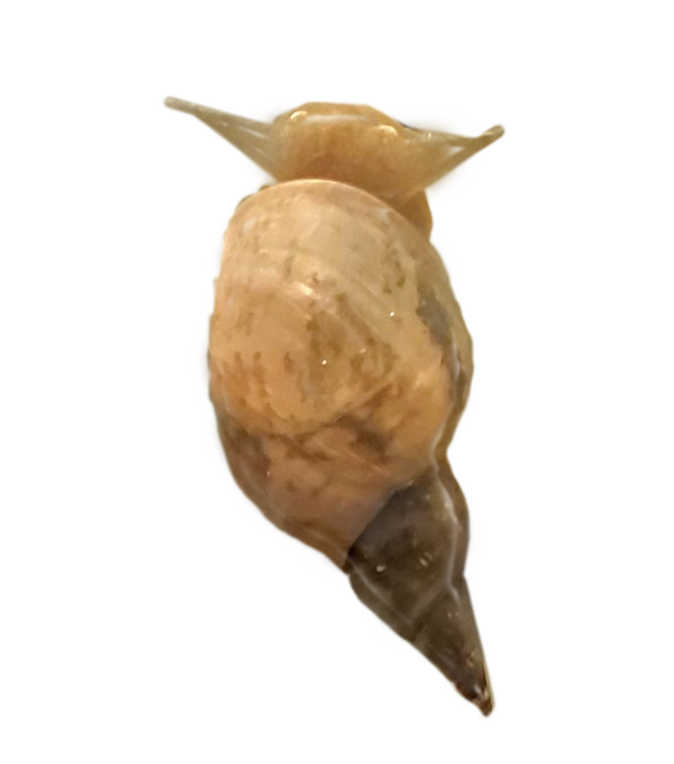
\includegraphics[width=\linewidth]{img/intro/lymnaea.png} 
		\caption{Imagen of \textit{Lymnaea Stagnalis}}
		\label{fig:snail spanish}
	\end{minipage}
	\hfill
	\begin{minipage}{0.65\textwidth}
		\centering
		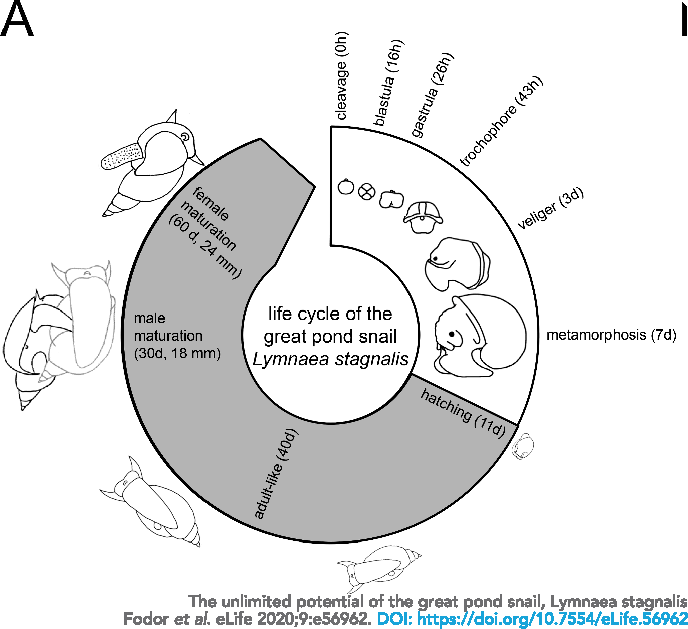
\includegraphics[width=\textwidth]{img/intro/lymnaea_life_cycle.pdf}
		\caption{Represnetación del ciclo de vida de \textit{L. stagnalis}. Figura 2A de \textcite{fodor_unlimited_2020} (\href{http://creativecommons.org/licenses/by/4.0/}{Creative Commons license}).}
		\label{fig:lymnaea_life_cycle spanish}
	\end{minipage}
\end{figure}


Además de estos estudios, ha sido clave en otros campos como el huésped-parásito o la edición del genoma. Este último campo se debe al ciclo de vida corto y bien estudiado en \textit{L. stagnalis} (ver Fig. \ref{fig:lymnaea_life_cycle spanish}), así como a la facilidad para criarlos en laboratorio, sin perder sus principales características a lo largo de las generaciones \parencite{noland_observations_1946}. Las grabaciones y análisis en este trabajo están enmarcados en el estudio de la actividad neuronal en su sistema nervioso central (SNC). El SNC de \textit{L. stagnalis} está compuesto por 11 ganglios que conforman el sistema: pares simétricos de ganglios bucal, pedal, cerebral, pleural y parietal, y un solo ganglio visceral (ver Sec. \ref{sec:lymnaea morphology}). Nos centraremos especialmente en su circuitp CPG alimentario, que mediante una combinación distribuida de neuronas motoras e interneuronas ubicadas principalmente en los ganglios bucales y cerebrales, produce un patrón rítmico de movimiento que permite la alimentación en tres fases (protracción, raspado y deglución). Además de este estudio del CPG, trabajaremos en las neuronas gigantes ubicadas en el ganglio parietal derecho (RPG), mejorando la actividad de alto voltaje (hasta 80mV) y lenta (30 a 100 ms por pico) para analizar en detalle la dinámica del potencial de acción.

\section{Estimulación neuronal}
\subsection{Técnicas de estimulación}

La estimulación neuronal ha sido un aspecto esencial en el estudio de la dinámica neuronal, permitiendo la modulación del sistema nervioso para explorar, reproducir y alterar su dinámica para su estudio. Hay varias técnicas para producir la estimulación, que podríamos clasificar en químicas --utilizando componentes químicos para bloquear/mejorar los mecanismos neuronales--, eléctricas --inyectando corriente en la membrana celular o los nervios-- u ópticas --donde se estimulan neuronas o circuitos a través de un proceso de iluminación. En esta tesis, nos centraremos en las dos últimas. En las técnicas eléctricas, desde las primeras aplicaciones de electrofisiología por \textcite{neher_singlechannel_1976} y la posterior aparición de la técnica de \textit{patch-clamp} \textcite{hamill_improved_1981}, se han desarrollado numerosas técnicas diferentes para distintos sistemas. El \textit{voltage-clamp }y el \textit{patch-clamp} modificaron el paradigma en la fisiología y la medicina básica en el estudio de la dinámica de la membrana celular con un detalle excepcional que todavía hoy dirige rangos de grabación y estimulación precisos \parencite{hamill_improved_1981}. A la técinca de \textit{voltage-clamp} le siguieron variaciones como el \textit{dynamic-clamp}, que mejora las posibilidades de electrofisiología combinándolo con las posibilidades de computación a través de un protocolo de bucle cerrado en tiempo real \parencite{nowotny_dynamic_2022}. Esto permite implementar algoritmos específicos para intervenir en la actividad neuronal y probar diferentes enfoques \parencite{chamorro_generalization_2012}. En cuanto a la estimulación óptica, una técnica novedosa y ampliamente utilizada es la optogenética, que mediante la modificación genética de los animales, hace que las neuronas sean reactivas a la luz y ha tenido grandes logros en las últimas décadas utilizando tanto para la estimulación como para la exploración y visualización de la actividad \parencite{chen_roles_2022}. Otro ejemplo aún en estudio es el láser infrarrojo cercano, una técnica novedosa que se explorará en detalle a lo largo de esta tesis. Esta técnica ha demostrado su potencial para la estimulación neuronal en diferentes sistemas como el hipocampo \parencite{liang_temperaturedependent_2009}, ganglios espinales en la cóclea \parencite{goyal_acute_2012, barrett_pulsed_2018, brown_thermal_2020} y otros sistemas \parencite{shapiro_infrared_2012, cayce_infrared_2014, begeng_activity_2022}.

\subsection{Neuromodulación y su necesidad para aplicaciones clínicas}

Más allá de la necesidad de la estimulación neuronal en la investigación básica para comprender y explorar la señalización y dinámica del cerebro, hay un impacto social directo para la estimulación neuronal en aplicaciones clínicas. En este contexto, la neuromodulación es un área de la medicina que involucra muchas especialidades y que puede definirse como "la ciencia de cómo las intervenciones eléctricas, químicas y mecánicas pueden modular las distintas funciones del sistema nervioso [y es] inherentemente no destructiva, reversible y ajustable" \parencite{krames_neuromodulation_2009}. Este campo es tan importante debido a sus posibilidades en el tratamiento de trastornos cerebrales, tanto por estimulación funcional como por la modulación a largo plazo a través de la plasticidad neuronal. La neuromodulación puede clasificarse, según la tecnología utilizada, como invasiva o no invasiva. Las tecnologías invasivas son aquellas que requieren una interacción directa con el sistema vivo, lo que causa daño, por ejemplo, incluyendo la cirugía. Un ejemplo conocido de este tipo es la estimulación cerebral profunda (DBS), esta técnica se ha utilizado de manera efectiva para tratar trastornos del movimiento al estimular eléctricamente el cerebro en ciertas áreas cerebrales después de implantar un dispositivo \parencite{limousin_longterm_2019, hariz_deep_2022}. En el caso de la neuromodulación no invasiva, podemos encontrar la estimulación magnética transcraneal (TMS), que mediante campos eléctricos estimula ciertas áreas del cerebro, exitosa, por ejemplo, en el tratamiento de la depresión o el trastorno obsesivo compulsivo \parencite{valero-cabre_transcranial_2017, clarke_patients_2018}. Cada tipo de técnica tiene sus propias ventajas, las técnicas invasivas suelen ser más precisas en espacio y tiempo, mientras que las técnicas no invasivas ofrecen más flexibilidad y adaptabilidad a diferentes pacientes y la difusión de la técnica. En este contexto, las técnicas ópticas discutidas para la estimulación en la investigación básica también han aumentado en popularidad para aplicaciones clínicas.
